\subsection{Concept}
	\begin{frame}
		\frametitle{Une problématique}
		Comment permettre aux utilisateurs de partager l'information, tout en les empêchant de se marcher dessus ?
		\begin{figure}
		\centering
		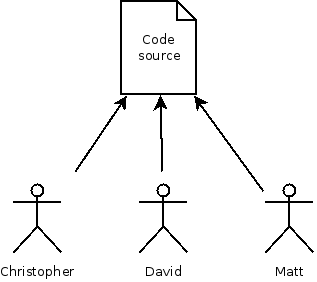
\includegraphics[width=50mm]{./Img/AccesConc.png}
		% AccesConc.png: 0x0 pixel, 0dpi, 0.00x0.00 cm, bb=
		\caption{Différents Docteurs veulent acceder à la source}
		\end{figure}
	\end{frame}
	
	\begin{frame}
		\frametitle{Une solution}
		\framesubtitle{La gestion de version (ou Version Control)}
		\begin{block}<1->{D\'efinition}
			La gestion de version consiste à maintenir l'ensemble des version d'un ou plusieurs fichier.
		\end{block}

		\begin{exampleblock}<2>{}
			\begin{figure}
				\centering
				\includegraphics<2>[width=50mm]{./Img/VersionsFich.png}
				% Diagramme1.png: 0x0 pixel, 0dpi, 0.00x0.00 cm, bb=
				\caption{\only<2>{Différentes version d'un fichier}}
			\end{figure}
		\end{exampleblock}		
	\end{frame}

	\begin{frame}
		\frametitle{Une solution}
		\framesubtitle{Le gestionnaire de version}
		\begin{itemize}
			\item <1->  Un gestionnaire de version est un système qui enregistre l'évolution d'un fichier au cours du temps.
			\item <2-> Ce système permet de récupérer à tout moment une version antérieure du fichier.
		\end{itemize}
	\end{frame}

	\begin{frame}
		\frametitle{Une solution}
		\framesubtitle{Exemple}
		\begin{figure}
			\centering
			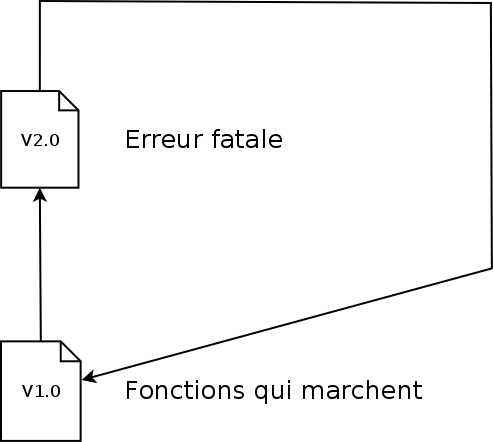
\includegraphics[width=60mm]{./Img/RevertFich.png}
			% Diagramme1.png: 0x0 pixel, 0dpi, 0.00x0.00 cm, bb=
			\caption{Récupération de la  version 1.0 d'un fichier}
		\end{figure}
	\end{frame}



\subsection{Notions}
	\begin{frame}
		\frametitle{Les types de gestionnaires de version}
		\begin{itemize}
			\item<1,2> Les gestionnaires centralisés \only<2>{: CVS, SVN}
			\item<3-> Les gestionnaires décentralisés \only<4->{: GNU Arch, Mercurial, Git}
		\end{itemize}
	\end{frame}


	\begin{frame}
	\frametitle{Version}
		\begin{block}{Définition}
			La version d'un fichier est l'avancement des modification d'un fichier qui a été validé par l'utilisateur.
		\end{block}
	\end{frame}

	\begin{frame}
		\frametitle{Branche}
		\begin{block}{Définition}
			Une branche est une version d'un projet que l'on souhaite continuer de manière indépendante 
		\end{block}
		\begin{figure}
			\centering
			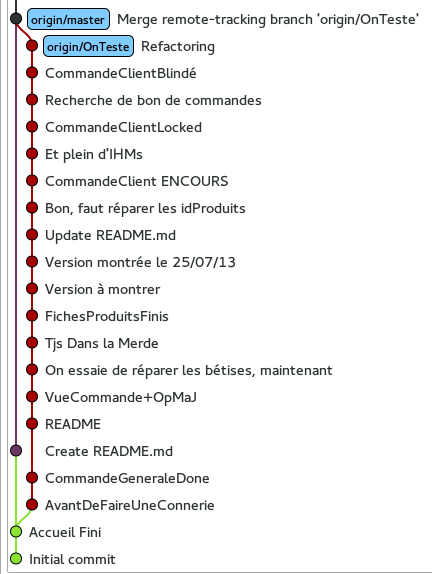
\includegraphics[width=35mm]{./Img/DefBranches.png}
			% DefBranches.png: 0x0 pixel, -2147483648dpi, nanxnan cm, bb=
			\caption{Un début de projet}
		\end{figure}
	\end{frame}